
\chapter{Results}
Several computational experiments have been performed to analyze the performance of the novel MGA approach developed in this project, and to study the techno-economic model of Europe presented. Initially the results of a study performing regular optimization of the techno-economic model of Europe is presented, providing a basic insight in the techno-economic model used. Knowing the optimal solutions to the optimization problem, the results of a study implementing the novel MGA method presented in this project, are presented. This study seeks to investigate how the installed capacities of the different technologies are distributed across all near optimal feasible solution to the problem.
Yet another MGA study is performed, analyzing the interplay between energy production in south and north Europe. This study also seeks to investigate the limitations of the MGA algorithm, in terms of the maximum allowable variables included in the decision space considered by the MGA algorithm. 
In order to compare the usefulness of the novel MGA approach developed in this project, a study comparing the novel MGA approach with previously presented MGA approaches have been performed. The results of this study will be presented, highlighting benefits and disadvantages of a total of four different MGA approaches including the one presented in this project. 


\section{Optimal solutions}
Before any MGA studies are performed, the baseline performance of the techno-economic model must be established. This is done by performing classic optimization of the models in order to find the optimal solutions. 

Initially the model is optimized without introducing any $\text{CO}_2$ constraints, in order to establish a baseline for $\text{CO}_2$ emissions. The baseline $\text{CO}_2$ emissions measured in tonnes per year, acts as the reference for $\text{CO}_2$ reductions in other scenarios. It is important to perform this study as real world numbers on $\text{CO}_2$ emissions doesn't necessarily compare to the numbers found using this specific model. This is due to the fact that the model used in this project simplifies the complex energy grid of Europe by a great deal, hereby introducing a lot of uncertainty. It is therefore relevant to compare the performance of the model used in this project to the performance of the actual energy system. 

When the optimal solution for the model with no $\text{CO}_2$ constraints is found, a range of optimizations are performed with altering $\text{CO}_2$ constraints. The allowable $\text{CO}_2$ emissions are calculated as a percentage of the emission of the base scenario. A total of three $\text{CO}_2$ reduction levels was chosen to investigate being 50\%, 80\% and 95\% reduction compared to the base scenario. The objective of performing these optimizations is to investigate the effect of the $\text{CO}_2$ constraint on the model, before performing any MGA studies. 

%Before starting any MGA studies, it is important to investigate and understand the optimal solution of the problem at hand. In this section, the found optimal solutions of the model will be presented. A range of $\text{CO}_2$ constraints have been investigated, and as the $\text{CO}_2$ constraint is altered a new optimal solution is found, therefore four optimal solutions representing a business as usual scenario, a 50\% $\text{CO}_2$ reduction, a 80\% $\text{CO}_2$ reduction and a 95\% $\text{CO}_2$ reduction scenario will be presented. 

\begin{figure}[h]\centering
\begin{subfigure}{1\textwidth}
	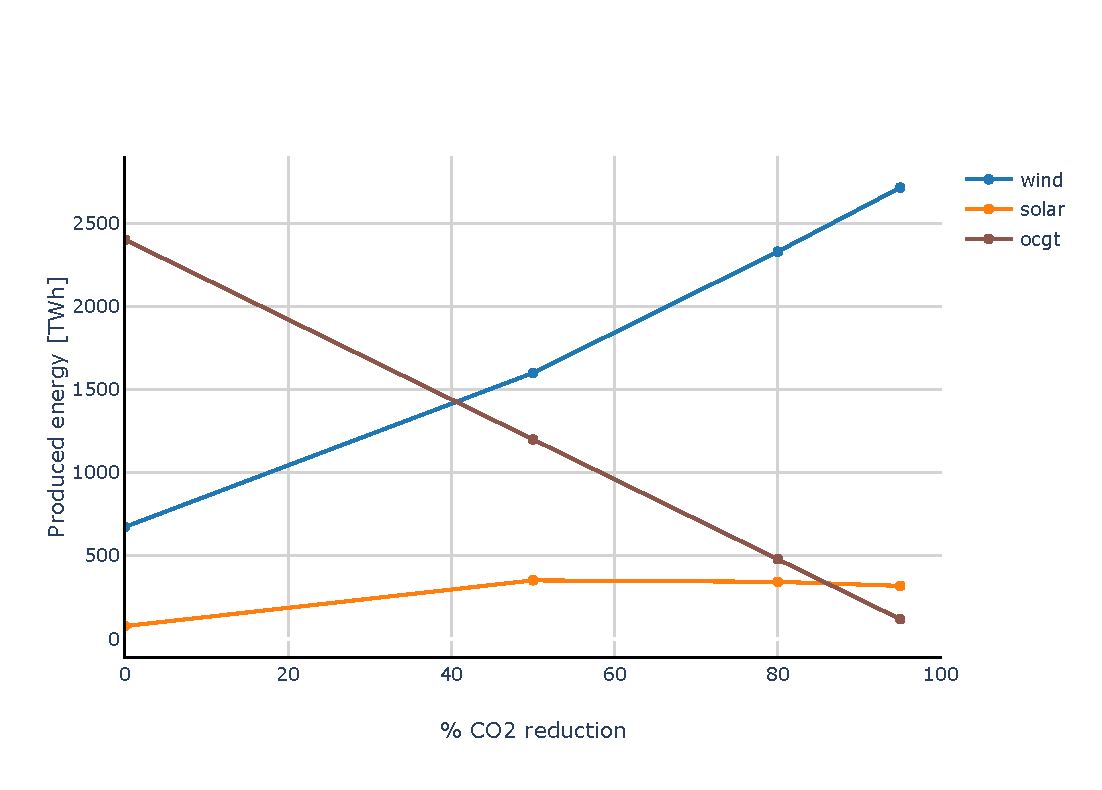
\includegraphics[width=.9\textwidth,trim={0 0cm 0cm 2.8cm},clip]{./Images/optimal_solutions_summary_production}
	\caption{}
	\label{fig:Optimal_Solutions_produc}
	\end{subfigure}%
\vspace{-10pt}
\begin{subfigure}{1\textwidth}
	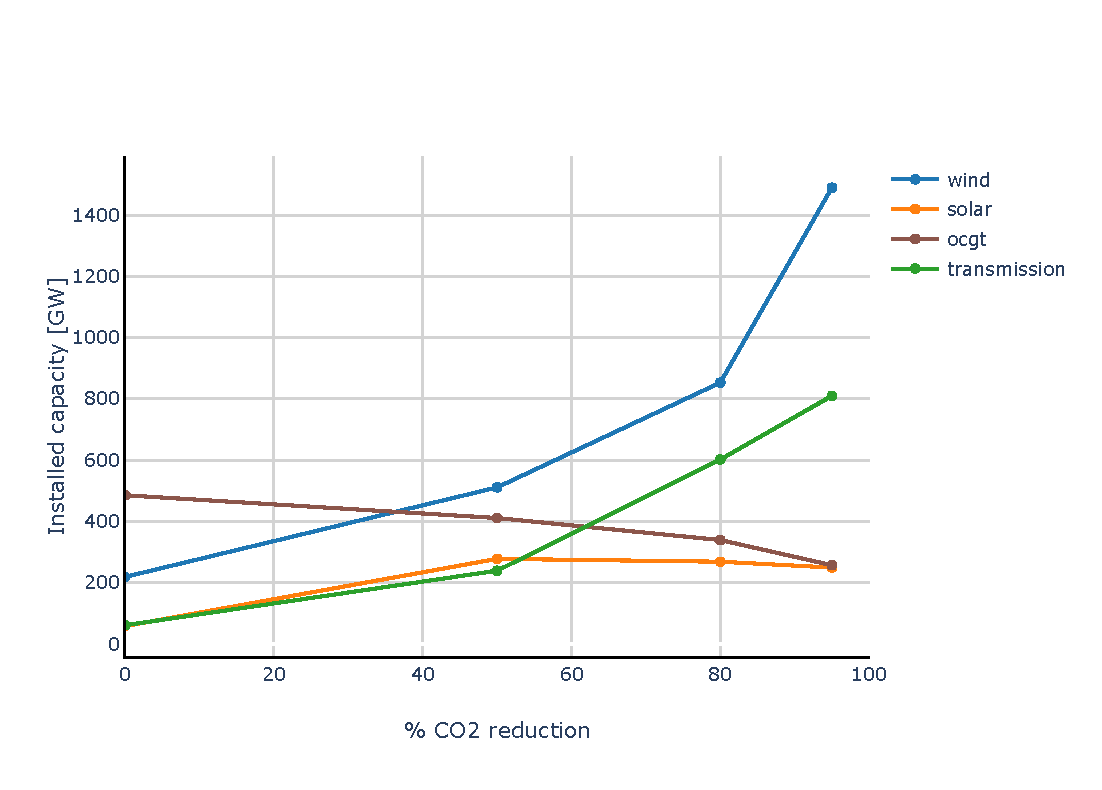
\includegraphics[width=1\textwidth,trim={0 0cm 0cm 2.8cm},clip]{./Images/optimal_solutions_summary}
	\caption{}
	\label{fig:Optimal_Solutions_summary}
\end{subfigure}%
\caption{Figure (a) shows the total amount of produced energy by the individual technologies during an entire year, for the four optimal solutions with different reductions in CO2 emissions. On figure (b) a summary of the total installed technology capacity versus \% $\text{CO}_2$ reduction for the four optimal solutions is presented.}
\label{fig:Optimal_Solutions_summary_both}
\end{figure}

\begin{table}[h]
	\begin{tabular}{lr|llll}
		Technology      & & Business as usual & 50\% $\text{CO}_2$  & 80\% $\text{CO}_2$  & 95\% $\text{CO}_2$  \\ \hline
	wind &[GW] & 219.1 & 511.2 & 853.3 & 1489.5 \\
	Solar &[GW]& 58.6 & 278.0 & 268.78 & 249.6 \\
	OCGT &[GW]& 485.5 & 411.2 & 339.4 & 257.2 \\
	Transmission &[GW]& 61.4 & 239.5 & 602.3 & 810.1 \\
	Gini coefficient & & 0.11 & 0.20 & 0.44 & 0.59 \\
	$\text{CO}_2$ emission &[MT] & 1151.9 & 576.0 & 230.4 & 57.6 \\
	Objective value &[1e9\euro] & 200.7 & 212.8 & 256.5 & 358.1 \\         
	\end{tabular}
	\caption{Key data from the four optimal solutions are presented.}
	\label{tab:Optimal_Solutions_summary}
\end{table}

On figure \ref{fig:Optimal_Solutions_summary}, the summarized technology capacities are presented, showing how the two $\text{CO}_2$ neutral energy sources increase as the $\text{CO}_2$ constraint is tightened. It is important to note how the installed wind capacity increases rapidly compared to solar PV that levels out, as the $\text{CO}_2$ reduction reaches the higher percentages. This could indicate that any further solar PV capacity would primarily generate surplus energy, as long as no storage technologies are implemented. Studies have previously shown that solar PV is highly dependent on short term storage if it is to be utilized on a larger scale \cite{rasmussen2011a} \cite{VICTORIA2019111977}. This is due to the high daily fluctuations in energy production from solar PV and therefore solar PV has a great synergy with short term storage technologies. 

Figure \ref{fig:Optimal_Solutions_summary} further shows that a wind solar mix of approximately 80\% wind and 20\% solar PV is desirable, when no storage solutions are implemented, if +90\% $\text{CO}_2$ reduction should be achieved. This complies very well with the results presented in \cite{rasmussen2011a}, where a study on the optimal wind and solar mix for Europe is performed. 

Comparing the produced energy in the four scenarios presented on figure \ref{fig:Optimal_Solutions_produc} with the installed capacities from figure \ref{fig:Optimal_Solutions}, it is seen how the energy produced by gas turbines drops drastically compared to the gas turbine capacity as $\text{CO}_2$ emissions are reduced. This means that every GW of installed OCGT capacity produces less energy in the scenarios with high $\text{CO}_2$ reduction. Instead of acting as primary energy source the gas turbines changes role and instead acts as backup capacity. The amount of produced energy from wind turbines compared to the installed capacity also seems to decrees when the $\text{CO}_2$ reduction increases above 80\%. This could indicate that after this point, additional installed wind capacity generates more surplus then previously installed capacity. 


The Gini coefficients for the four scenarios is presented in table \ref{tab:Optimal_Solutions_summary} and on figure \ref{fig:Gini}. The Gini coefficient expresses the equality in production versus consumption for the four scenarios. A low Gini coefficient indicates that energy is being produced locally and opposite, a high Gini coefficient indicates that energy is being produced away from where it is needed. The Gini coefficients of the four optimal solutions appears to increase, together with the capacity of wind and solar power, as the $\text{CO}_2$ constraint is tightened. This could suggest that it is beneficial to install wind and solar power in countries with good wind and solar profiles and then transmit the energy to countries with less favorable wind and solar profiles. Analyzing the average capacity factors for wind power on figure \ref{fig:capacity_factor}, it is seen that higher capacity factors are common in northern countries. This corespondents very well with where the large capacities of wind are placed in the optimal solutions subject to high $\text{CO}_2$ constraints presented on figure \ref{fig:Optimal_Solutions}c and \ref{fig:Optimal_Solutions}d. Comparing the installed capacities presented on figure \ref{fig:Optimal_Solutions} with the total demand of the individual countries presented in figure \ref{fig:demand}, it is clearly seen that as $\text{CO}_2$ emissions are reduced, the installed capacities moves further and further away from the countries with the largest demands. 

\begin{figure}[h]\centerfloat
	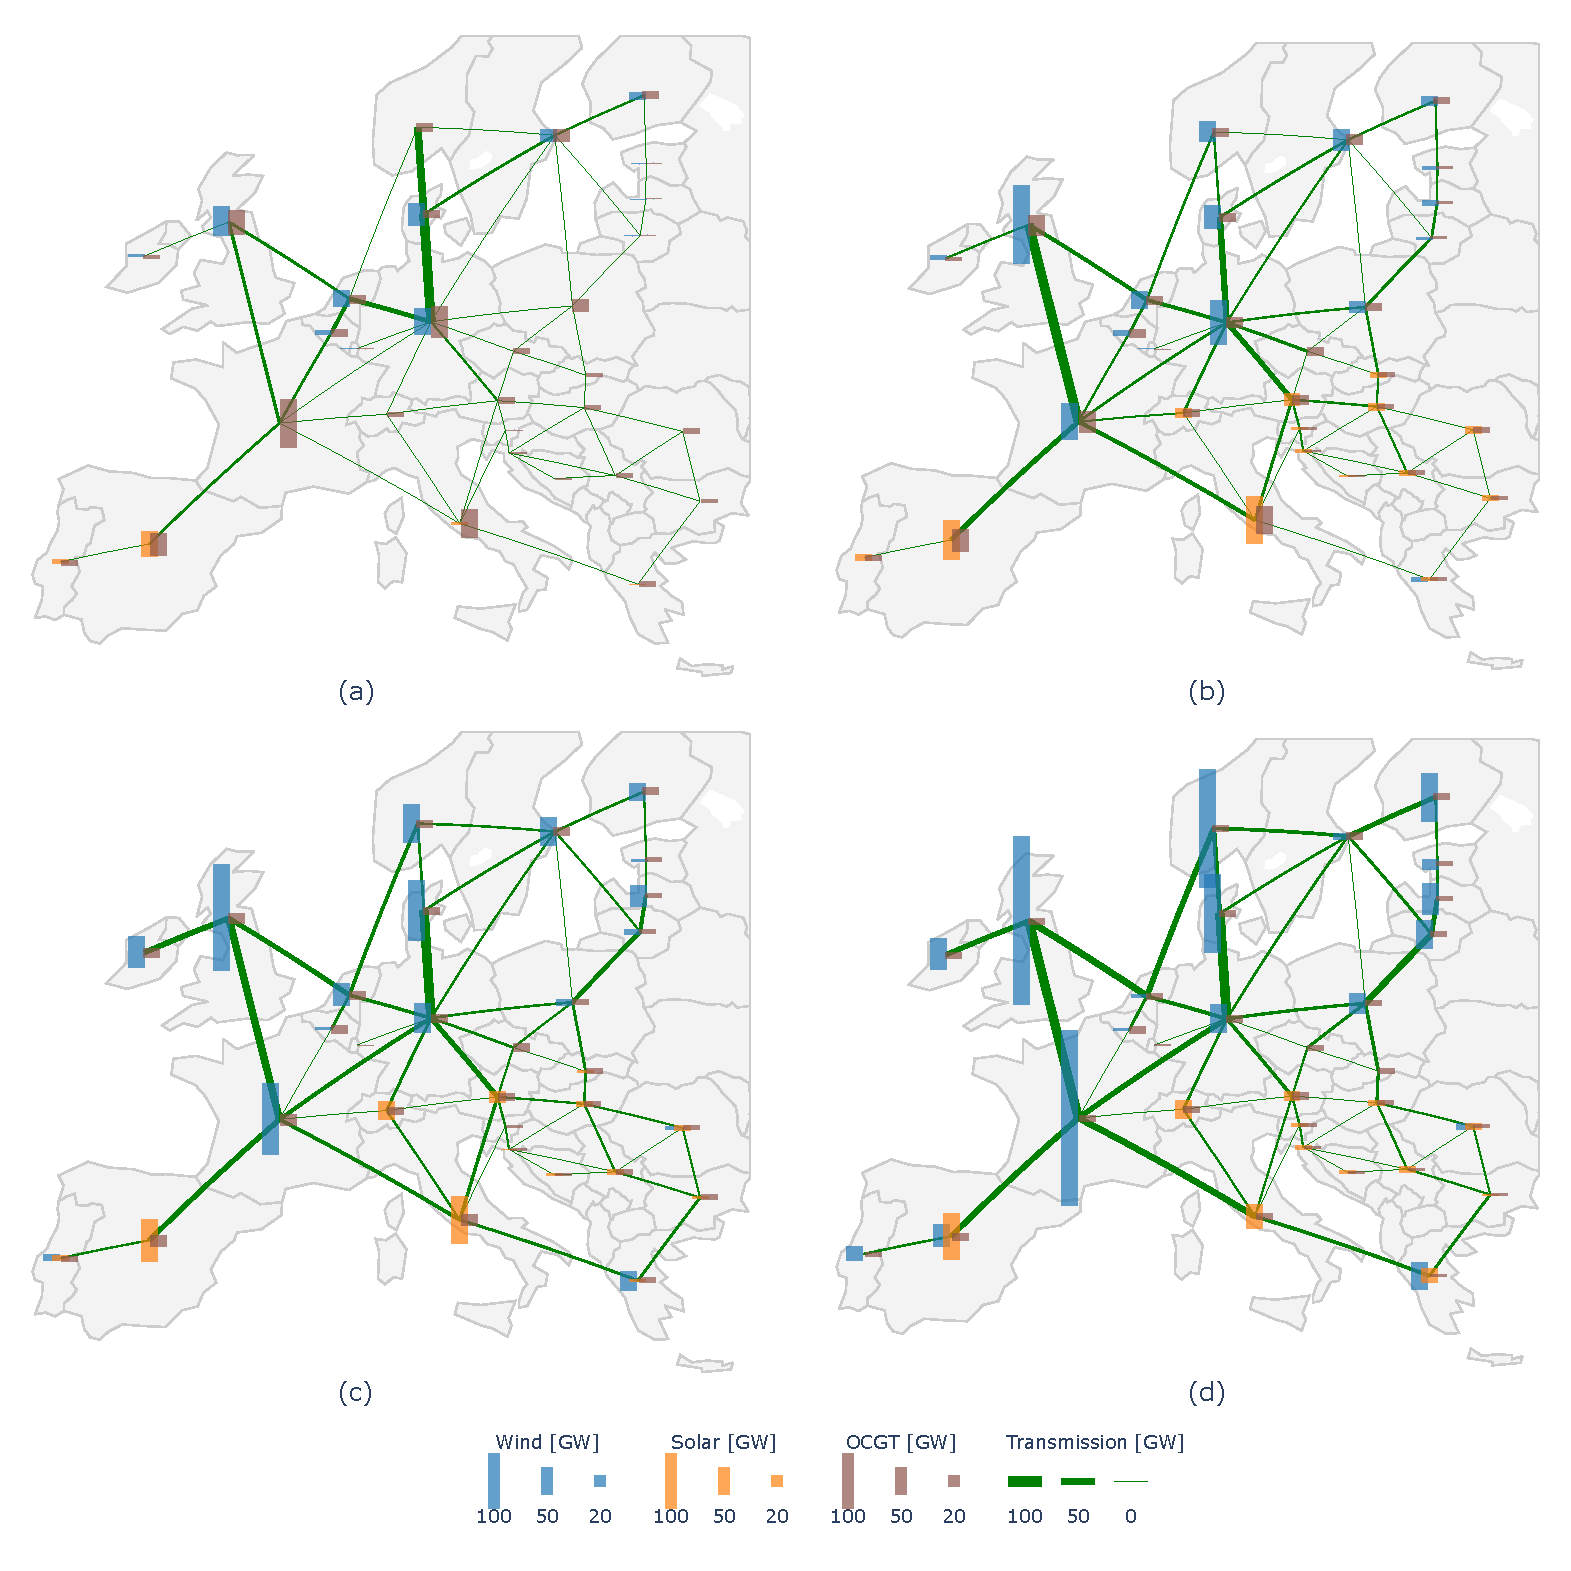
\includegraphics[width=1.1\textwidth]{./Images/Optimal_solutions}
	\caption{The figure presents the layout of technology capacities of all four optimal solutions. On figure (a) the business as usual scenario is presented, (b) shows data for the scenario with 50\% CO2 reduction, (c) 80\% reduction and (d) 95\% reduction in CO2 emissions.}
	\label{fig:Optimal_Solutions}
\end{figure}

\subsection{Business as usual}
In the business as usual scenario, seen on figure \ref{fig:Optimal_Solutions}a, where no constraint on the $\text{CO}_2$ emission is implemented, energy is primarily supplied by gas turbines as expected. Any significant capacities of variable renewable energy sources is only implemented in countries where the price of energy produced from such technologies can compete with the price of energy from gas turbines. Analyzing figure \ref{fig:capacity_factor} it is found that wind energy is favorable in the northern countries and solar energy only becomes favorable in the most southern countries, in this case Spain and Portugal. 
Furthermore, the energy generation is spread, fairly even across the network, thereby requiring less transmission capacities, and thereby also resulting in a fairly low Gini coefficient of 0.11. In this scenario transmission is purely installed between countries with significant shares of VRES. 

The $\text{CO}_2$ emission in the base scenario without $\text{CO}_2$ constraints was found to be 1151.9 MT $\text{CO}_2$/year, which complies reasonably well with the 2011 $\text{CO}_2$ emission for the EU-28 countries energy sector, found by the European Environment Agency (EEA) to be 1517.3 MT $\text{CO}_2$/year \cite{eea_co2_emission}. Although the numbers are off by some hundred MT $\text{CO}_2$/year, and the numbers from EEA only represent the EU-28 countries, this comparison can conclude that the model used in this project, despite its coarse spatial resolution and small number of included technologies, is capable of producing results with an acceptable accuracy. 


\subsection{Reduced $\text{CO}_2$ emission scenarios}

The distribution of installed capacities of the scenarios with reduced $\text{CO}_2$ emissions are presented on figure \ref{fig:Optimal_Solutions}b, c and d, with respectively 50, 80 and 95\% $\text{CO}_2$ reduction. All three scenarios implements wind energy in northern Europe and implements large amounts of transmission capacity between all countries with high shares of wind power. OCGT capacity appears to be evenly spread across the countries. Significant shares of solar power is only implemented in southern Europe, and even with a $\text{CO}_2$ reduction of 95\%, the most northern country to install solar power is Austria. 
As the $\text{CO}_2$ constraint is tightened, the Gini coefficient increases, as the countries with favorable conditions for solar and wind power, simply increases their capacity of these technologies. Whereas, technology capacities in less favorable countries stay unaffected. 

Looking at the scenario costs in table \ref{tab:Optimal_Solutions_summary}, it is seen that as the $\text{CO}_2$ constraint is tightened, the cost increases rapidly. From the business as usual scenario to the scenario with a 50\% reduction there is only an increase in price of 6\%. When the $\text{CO}_2$ emissions is to be reduced beyond this point, price increases rapidly, and to achieve a reduction of 95\% the cost almost double, having increased with 78\%, compared to the business as usual scenario. This also complies with the data shown in figure \ref{fig:Optimal_Solutions_summary_both}, where it can be seen that total installed production capacity increases, even though the energy demand stays the same. These result are very much in line with the results found in \cite{Gorm_Surplus}, where surplus electricity is investigated in scenarios with large shares of variable renewable energy sources. 

\section{MGA study of four dimensional decision space}\label{sec:4D}
The objective of this experiment is to document the performance of the techniques developed in this project, by studying the techno-economic model presented in chapter \ref{chap:model}. Focus is placed on the relevance/usability of the data extracted from the model using the newly developed technique, as well as shear performance measured in computation time. The experiment will explore the interplay between variable renewable energy sources and transmission on an international level spanning all countries in the model. 

In this experiment the decision space is reduced to just four dimensions by grouping the decision variables as explained in section \ref{sec:dim_reduction}. The four variables in the new decision space is the total amount of installed gas turbine (OCGT) capacity, wind turbine capacity, solar pv capacity and the total installed transmission capacity. Using a low dimensional space allows for a thorough exploration of the feasible space as a lower dimensional decision space, needs fewer computations per study, thereby reducing computation time. 

As a thorough exploration of the near optimal feasible space is desired, to evaluate the performance of the technique, combined with a desire to learn more about the features of the near optimal feasible space, a range of MGA studies is performed with varying parameters. 
For every single MGA exploration there are two parameters that can be altered. These are the amount of reduction in $\text{CO}_2$ emission compared to the base model, and the amount of MGA slack used. For this experiment it was chosen to iterate over both of these variables exploring $\text{CO}_2$ reductions of 0, 50, 80 and 95\%, and MGA slacks of 1, 2, 5, and 10\%. This means that a total of 16 MGA studies is to be performed. 

Even though it was established that multiplicity of sampled points has a large effect on the results, when a high dimensional space is reduced to one of much lower dimension, it has not been accounted for in this study, due to the added computing time needed. 


%- Very large range of possible configurations for VRES and Transmisison, OCGT more limited
%- OCGT has sharp lower limit
%- Solar power can be ommitted if desired
%- Tighter CO2 caps results in larger investement flexibility. As Fabian \cite{Fabian_MGA} unlike Price \cite{MGA_Price}

%In the first MGA study performed it was chosen to explore a four dimensional near optimal feasible space, with the four dimensions being total installed ocgt capacity, total installed wind capacity, total installed solar PV capacity and total installed transmission capacity. 

\begin{figure}[p]\centerfloat
	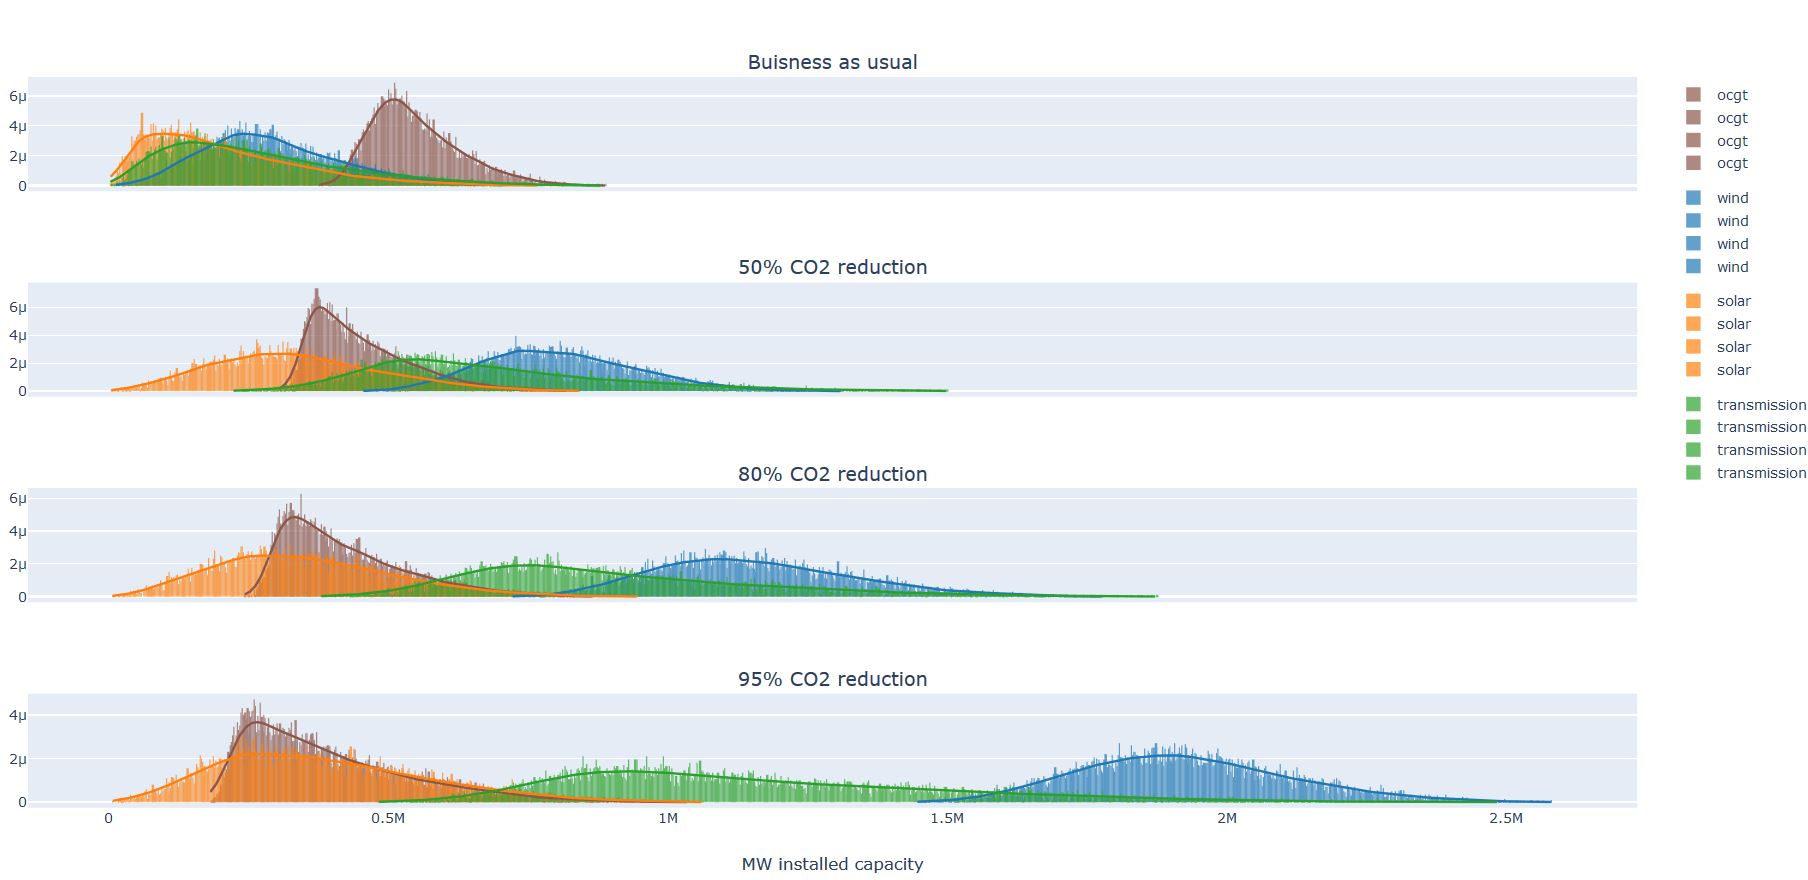
\includegraphics[width=1.2\textwidth,trim={0 1.5cm 0 0cm},clip]{./Images/4D_study_histogram}
	\caption{The figure shows the distribution of technology capacities for four MGA studies, where a MGA slack of 10\% have been used.}
	\label{fig:4d_hist}
\end{figure}


The distribution of capacities found in the four MGA studies is presented on figure \ref{fig:4d_hist}. As it was seen with the optimal solutions, the figure clearly shows how decreasing $\text{CO}_2$ emissions leads to an increase in wind and transmission capacity and a reduction in OCGT capacity. The results presented on figure \ref{fig:4d_hist}, furthermore provides information about the distribution of capacities. When analyzing the capacity distributions presented on \ref{fig:4d_hist} it is important to consider that there hasn't been accounted for multiplicity, meaning that the true distributions would be narrower, as discussed in section \ref{sec:Multiplicity}.

It is particularly interesting to see how the OCGT capacity distribution has a sharp lower bound, indicating that a rather fixed minimum amount of OCGT capacity is needed in all scenarios. The minimum OCGT capacity needed will be given by the remaining energy demand in the hour with the combined lowest availability of wind and solar power. In order to remove the need for backup generators such as gas turbines, would require unrealistically large capacities of wind and solar power. 

Figure \ref{fig:4d_hist} also shows how the distribution of capacities become wider as $\text{CO}_2$ emission is decreased. This essentially means that a larger configuration flexibility is available as $\text{CO}_2$ emissions is reduced. It could, however also be a result of how the MGA slack is defined. The MGA slack is defined as a percentage of the optimal solution scenario cost. As the cost of the optimal solutions varies a lot from the scenario with no $\text{CO}_2$ constraint to the scenario with tight $\text{CO}_2$ constraint, the allowable extra cost of scenarios also varies a lot, if measured in shear size and not as a percentage of the optimal solution objective value.

The distributions of solar power capacity in all four scenarios presented on figure \ref{fig:4d_hist}, all reach a value of 0 GW, meaning that solar power can be omitted if desired. In the scenarios with larger $\text{CO}_2$ reduction, this would however be a very extreme scenario, leading to a very specific design of the energy network. It is however not possible to configure a solution in a way that omits wind power in any of the four scenarios. 

\begin{figure}[h]\center
	\includegraphics[width=1\textwidth,trim={0 0cm 0 0cm},clip]{./Images/corelation_4D}
	\caption{This figure presents all variable correlations of the four MGA studies performed with 10\% MGA slack. Distributions of the four individual technologies are plotted on the diagonal, scatter plots of the data are shown in the lower left half and correlation values are presented in the upper right half of the plot matrix.}
	\label{fig:corelation}
\end{figure}

On figure \ref{fig:corelation} correlations of the four variables of the simplified decision space is shown. Data from all MGA studies performed have been used to generate this figure. 
The figure shows a strong correlation between wind power and transmission with a correlation of 0.50. This corresponds well with the results presented on figure \ref{fig:Optimal_Solutions}, where reinforcements on to the transmission grid is made as more wind is introduced to the model. Similar correlations between large shares of wind power and transmission capacity has been found in an article investigating this subject \cite{PURVINS20111461}. On the other hand, when analyzing the correlation between transmission and solar power a small negative correlation of -0.07 is found. This could suggest that the solar capacities installed, only produce enough energy to supply the country wherein they are installed, and therefore a need to transmit electricity generated by solar power doesn't exist. The correlation between energy production from solar PV in different countries has been studied in \cite{SolarPV_transmission}, where a strong correlation between production periods was found. As sunrise and sunset are similar in all European countries, the production of energy from solar PV happens simultaneously across entire Europe. Therefore an increase in transmission capacity would not allow more solar PV capacity to be installed. These results from \cite{SolarPV_transmission}, corresponds very well with whats seen in this project. 
A very strong negative correlation between OCGT and transmission is also presented on figure \ref{fig:corelation} with a correlation of -0.33. The capacity factor of OCGT does not depend on geographically determined factors and therefore OCGT capacity is installed where it is needed, leading to a negative correlation with transmission capacity.  
Another strong negative correlation is between wind power and OCGT with a value of -0.33. These two technologies appear to compete somewhat equally as energy sources.  


Analyzing the correlations of a single MGA study, namely the one with a $\text{CO}_2$ constraint of 95\% presented on figure \ref{fig:corelation_2}, it is a completely different story. Here the most significant correlation is between wind and solar power, that has a negative correlation of -0.72. This indicates that when a specific $\text{CO}_2$ reduction is desired, wind and solar power competes evenly as energy generating technologies. 
It is interesting to see how wind power and transmission has a small negative correlation when the correlations are calculated for just a single MGA study, compared to the large positive correlation, when data from all scenarios was considered. 


\begin{figure}[h]\center
	\includegraphics[width=1.\textwidth,trim={0 0cm 0 0cm},clip]{./Images/corelation_4D_95}
	\caption{The figure shows all variable correlations of the MGA study with a $\text{CO}_2$ emission reduction of 95\%. Distributions of the four individual technologies are plotted on the diagonal, scatter plots of the data are shown in the lower left half and correlation values are presented in the upper right half of the plot matrix.}
	\label{fig:corelation_2}
\end{figure}

In this project cost have been treated as one combined cost for the entire European energy network. This is however a very large simplification of the problem. In reality energy system cost is treated on national level, and therefore it is desired to distribute the energy system cost as evenly across all countries in the model. In this project the Gini coefficient is used as a measure for the equality of energy production versus consumption. This Gini coefficient can also be used as a measure of the equality in the distribution of system cost. 


\begin{figure}[h]\centering
	\begin{subfigure}{1\textwidth}
		\includegraphics[width=.9\textwidth,trim={0 0.8cm 0 2.5cm},clip]{./Images/corelation_gini_co2}
		\caption{}
		\label{fig:gini_co2}
	\end{subfigure}%
	\vspace{-.5cm}
	\begin{subfigure}{1\textwidth}
		\includegraphics[width=1\textwidth,trim={0 0.8cm 0 2.5cm},clip]{./Images/corelation_mix_co2}
		\caption{}
		\label{fig:mix_co2}
	\end{subfigure}%
	\label{fig:derivative_correlations}
	\caption{Figure (a) plots the Gini coefficient versus the reduction in $\text{CO}_2$ emissions. Figure (b) plots the wind/solar mix $\alpha$ versus the reduction in $\text{CO}_2$ emissions.}
\end{figure}

On figure \ref{fig:gini_co2} the Gini coefficient for all studies performed in this experiment is plotted against the $\text{CO}_2$ reduction. On the figure it is seen that there is a very strong positive correlation between $\text{CO}_2$ reduction and the Gini coefficient. This means that as requirements to reductions in $\text{CO}_2$ emissions increase, more energy needs to be produced in outside the countries where it is needed. A larger Gini coefficient also means that some countries will have to invest more money in modernizing the energy grid by installing larger capacities of renewable energy sources, and other countries will be depending on import of energy from countries with large capacities of renewable energy. As a country it is desired to be self sufficient with energy as energy is one of the most critical resources. The desire to reduce the Gini coefficient might therefore introduce a larger financial willingness. On figure \ref{fig:gini_co2}, it is seen that a 1\% slack on total system cost requires a Gini coefficient of at less 0.5 for a $\text{CO}_2$ reduction of 95\%, but increasing the slack to 10\% allows for a Gini coefficient as low as 0.3 for the same reduction in $\text{CO}_2$ emissions.  

In this study, the only variable renewable energy sources included are the two major variable renewable energy technologies, wind and solar power. From the correlation plot on figure \ref{fig:corelation}, as slight negative correlation with a value of -0.11 was seen. Such a small correlation value indicates that these two technologies interfere very little with each other, and that the share of wind and solar power remain somewhat constant. On figure \ref{fig:mix_co2}, the share of wind and solar power is plotted against $\text{CO}_2$ emissions. The share of wind and solar power $\alpha$ is calculated as the wind capacity relative to the total capacity of variable renewable energy. 

\begin{equation}
	\alpha =  \frac{\text{wind capacity}}{\text{wind capacity}+\text{solar capacity}}
\end{equation}

On figure \ref{fig:mix_co2} it is seen that the wind solar mix has an average around 0.8, complying very well with the results from \cite{rasmussen2011a}, where the mix of wind and solar power was studied. The penetration of wind power increases as $\text{CO}_2$ emissions decrease, which complies well with the results seen in the optimal solutions on figure \ref{fig:Optimal_Solutions_produc}, where implementation of solar PV capacity stagnates at $\text{CO}_2$ reduction levels higher than 50\%. Figure \ref{fig:mix_co2}, further shows that with a slack of 10\% on total system cost a wide span is available in the wind solar mix. At 95\% $\text{CO}_2$ reduction, it is possible to have a scenario that is 100\% wind dominated or a scenario where 50/50 mix between wind and solar is used. 

Having analyzed the results from this experiment, it can be concluded that the developed MGA algorithm is capable of providing useful insights regarding the techno-economic model investigated. Information that would not have been made available with other methods was extracted allowing for great insights regarding the possibilities available within the near optimal feasible space. 

\section{MGA study using seven decision variables}\label{sec:7D}
In the previous experiment, variables was grouped by technology type. It is however possible to group the variables in any way desired. Therefore a study investigating the interplay between energy production in North and South Europe has been performed, grouping the variables not only by technology type, but also by spatial location. A total of 7 grouped variables is formed, including OCGT, wind and solar power from both north and south Europa, and the total amount of transmission capacity. The grouped variables then becomes: 

\begin{equation*}
 \mathbf{x} = 
 \begin{Bmatrix}
 	x_1:& \text{North OCGT} \\
 	x_2:& \text{North wind} \\
 	x_3:& \text{North solar} \\
 	x_4:& \text{South OCGT} \\
 	x_5:& \text{South wind} \\
 	x_6:& \text{South solar} \\
 	x_7:& \text{Transmission} 
 \end{Bmatrix}
\end{equation*}

\begin{figure}[h]\centering
	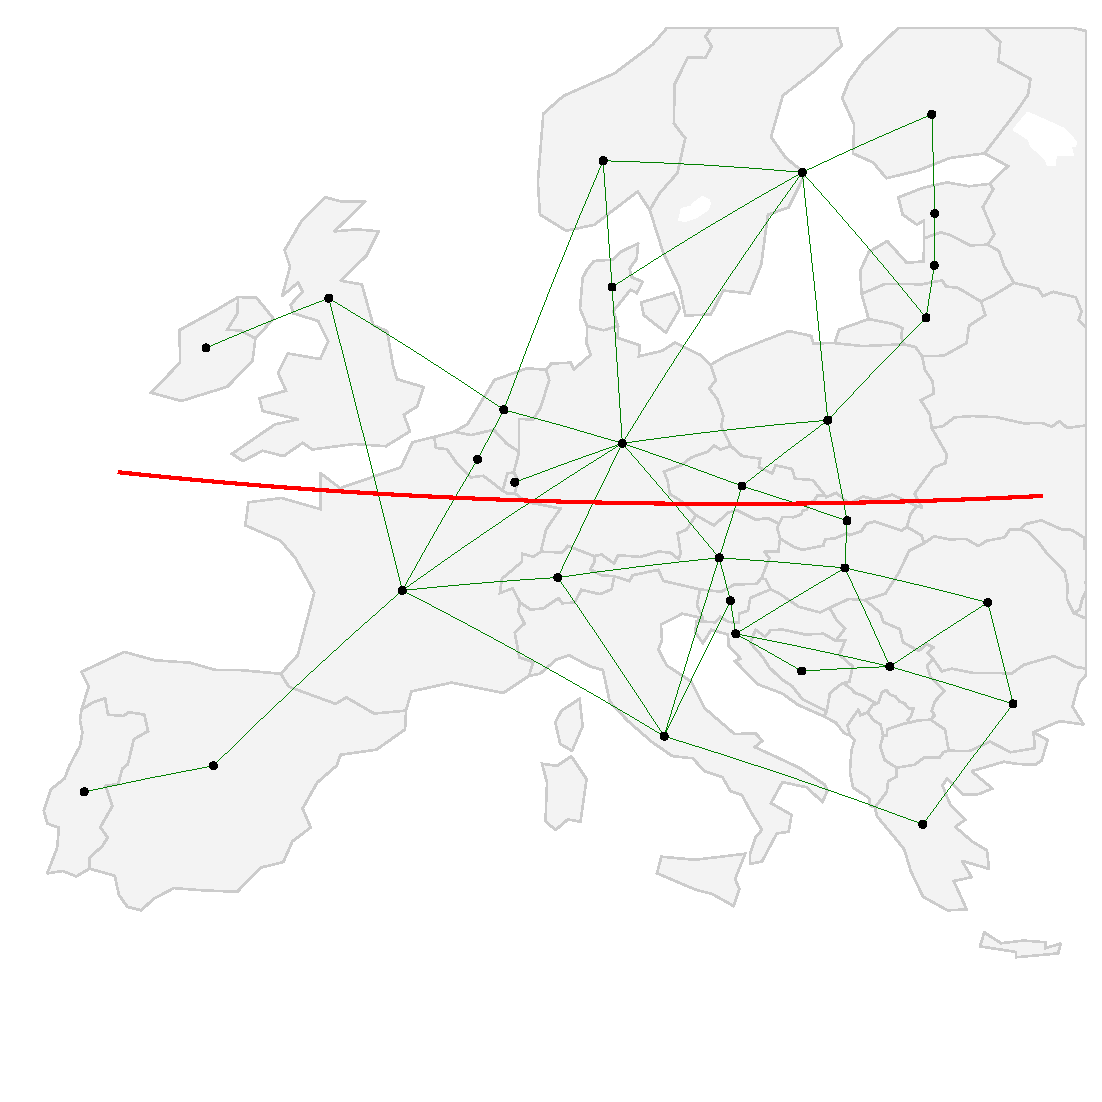
\includegraphics[width=.7\textwidth,trim={0 3cm 0 0cm},clip]{./Images/7D_study_topology}
	\caption{The figure shows the topology of the techno-economic model used in the study. The red line indicates the parting line between north and south Europe. }
	\label{fig:7d_topology}
\end{figure}

A parting line between north and south Europe was drawn at latitude 49.2421, which is equivalent to the median of the latitude position of all country centroids included in the model. All countries with a centroid north of latitude 49.2421 is considered as north Europe, and all other countries are considered as south Europe. A total of 15 countries are included in each category. The parting line is presented on figure \ref{fig:7d_topology}. 

\begin{figure}[p]\centerfloat
	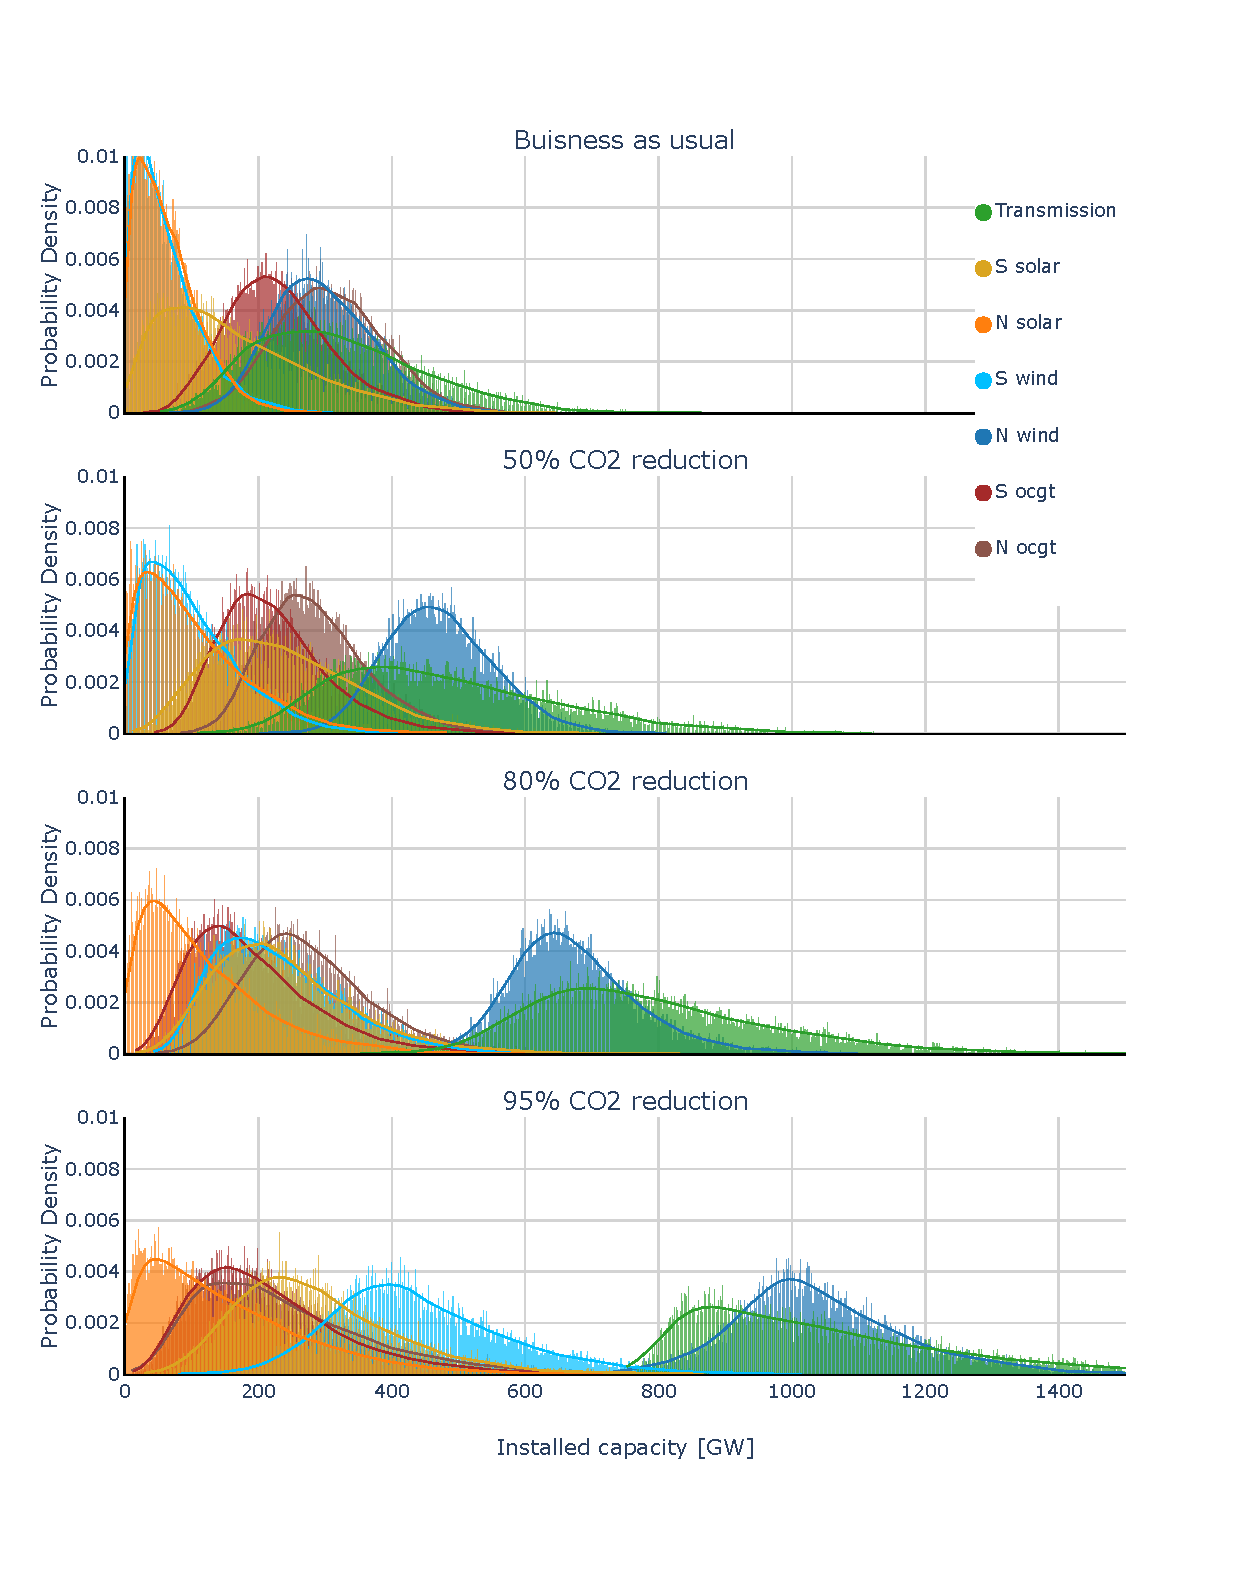
\includegraphics[width=1.3\textwidth,trim={0 1.7cm 0 0cm},clip]{./Images/7D_study_histogram}
	\caption{The figure shows the distribution of technology capacities for four MGA studies, where a MGA slack of 10\% have been used, and seven variables has been included in the MGA study. }
	\label{fig:7d_hist}
\end{figure}

Using the novel MGA method presented in this project, the capacities of all near optimal solutions was found, using a MGA slack of 10\% on four scenarios with respectively 0, 50, 80 and 95\% reduction in $\text{CO}_2$ emissions. 

On figure \ref{fig:7d_hist}, a histogram presenting all seven grouped variables for all four scenarios is shown. Much like the study performed using only four grouped variables seen on figure \ref{fig:4d_hist}, the wind and solar capacities increase as $\text{CO}_2$ emissions are reduced.  
Analyzing the data presented on figure \ref{fig:7d_hist}, it is clearly seen that wind power in northern Europe is preferred over any other energy generating technologies, as $\text{CO}_2$ emissions are lowered. Comparing solar power in north and south Europe, it is seen that south Europe in all scenarios have a larger amount of installed capacity. Scenarios where large shares of solar power is installed in north Europe is however also feasible, and in a scenario where $\text{CO}_2$ emissions are reduced by 95\%, a scenario with 600GW of installed solar capacity in north Europe wold be feasible. 

Analyzing the distributions of wind and solar power on figure \ref{fig:7d_hist}, it is seen that there is an overlap between respectively wind in north and south Europe, and solar power in north and south Europe. This shows, that a scenario with more solar capacity in northern Europe compared to south Europe is feasible with a 10\% slack on cost, or a scenario with more wind in southern Europe than northern Europe. 

Analyzing the correlations presented on figure \ref{fig:7d_corr}, results show a significant correlation between wind and transmission. Especially wind in north Europe has a strong correlation with transmission, with a correlations above 0.4. Wind power in south Europe correlates positive with transmission too, only with a correlation factor of 0.12. 
The results presented on figure \ref{fig:7d_corr}, further shows strong negative correlations between OCGT in north and south Europe, indicating that OCGT in north Europe competes very directly with OCGT power in south Europe. A similar tendency is seen between solar power in north and south Europe. Interestingly, no correlation is seen between wind in north and south Europe, indicating that the installed capacity of wind in either end of Europe, has no effect on each other. 

\begin{figure}[h]\centerfloat
	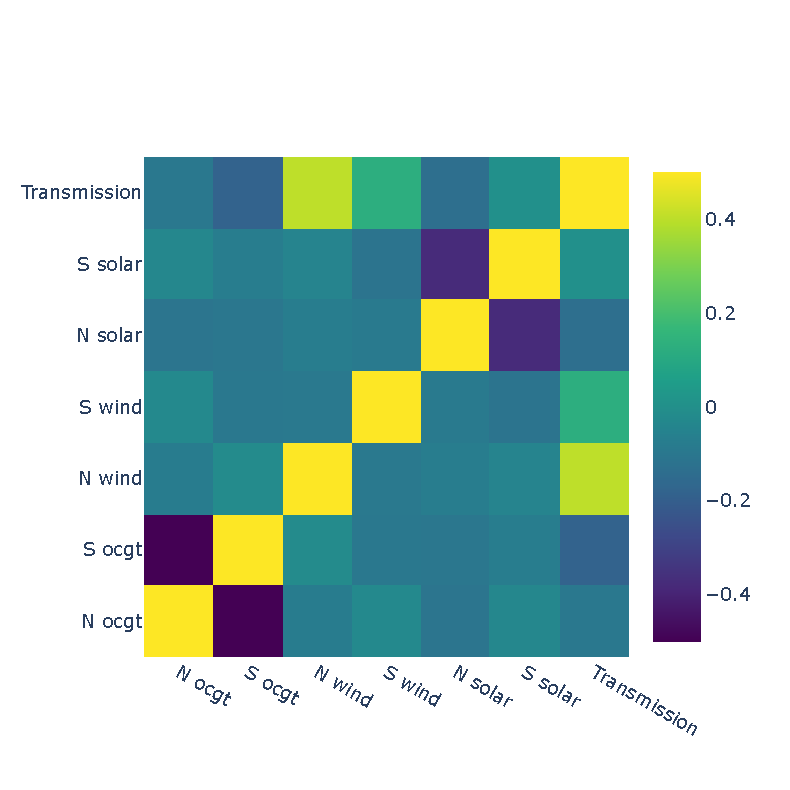
\includegraphics[width=0.8\textwidth,trim={0 .5cm 0 2cm},clip]{./Images/7D_study_corr}
	\caption{The figure shows a heatmap representing the correlation matrix of the variables in the four MGA studies performed with seven variables included in the study.}
	\label{fig:7d_corr}
\end{figure}

Each of the four studies performed in this experiment required 48 hours of computing time on the PRIME computing cluster \cite{Prime} using a single 32 core computing node. Including more variables in the decision space considered by the MGA algorithm is possible but the practical maximum is estimated to be roughly 10 decision variables.  

\section{Comparison of MGA algorithms}\label{sec:MGA_comparisons}
The goal of this experiment is to highlight the benefits and weakness of existing MGA methods compared to the novel MGA approach presented in this project. The following four different MGA techniques will be explored: The HSJ approach presented in \cite{DeCarolis_MGA}, an approach where groups of variables are maximized and minimized presented in \cite{Fabian_MGA} together with an approach where all decision variables are maximized and minimized and the novel approach presented in this project. 

\begin{figure}[h]\centering
	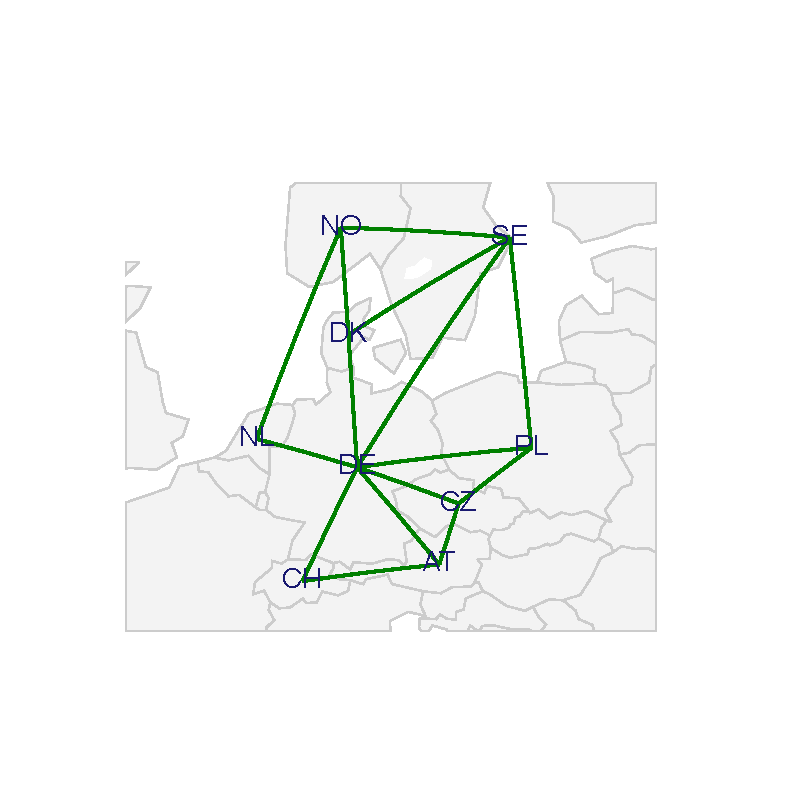
\includegraphics[width=.7\textwidth,trim={0 2.8cm 0 3cm},clip]{./Images/comparison_topology}
	\caption{The figure shows the topology of the simplified network used in study comparing performance of MGA algorithms. }
	\label{fig:comparison_topology}
\end{figure}


When comparing MGA approaches in this section, it is very important to keep in mind what to goal of performing an MGA analysis is, and what measure characterized a good MGA technique. The overall objective is to explorer the possibilities for alternative solutions to the optimization problem within a certain range of economical slack. Solutions to an techno-economic problem as the one considered in this project can however be different in a wide range of manners, as the decision space is high dimensional. This makes it hard to determine the coverage of the decision space for a given MGA method, as the extend of the decision space is unknown. Instead, the results found with the different MGA methods, will be analyzed, compared and discussed in an attempt to determine strengths, and weaknesses for the MGA methods. 

In order to generate comparable results, all four MGA methods are implemented on the same simplified network. As the focus of this experiment is to compare methods, and not to analyze an techno-economic model, a simplified model is used to reduce computation time needed, and complexity of the results. The techno-economic model used in this experiment includes only nine of the thirty countries from the full model as shown on figure \ref{fig:comparison_topology}. Furthermore, only a single 24 hour period is simulated. The result is a model with 27 variables (9 countries with 3 technologies each), when hourly dispatch is not considered as a decision variable. Furthermore, a $\text{CO}_2$ constraint is employed forcing the model to reduce $\text{CO}_2$ emissions with 80\% compared to an unrestricted scenario. 

\begin{figure}[h]\centering
	\begin{subfigure}{.5\textwidth}
		\includegraphics[width=1.\textwidth]{./Images/Comparison_1}
		\caption{}
		\label{fig:comparison_1}
	\end{subfigure}%
	%\vspace{10pt}
	\begin{subfigure}{.5\textwidth}
		\includegraphics[width=1.\textwidth]{./Images/Comparison_4}
		\caption{}
		\label{fig:comparison_2}
	\end{subfigure}%
	\vspace{1pt}
	\begin{subfigure}{.5\textwidth}
		\includegraphics[width=1.\textwidth]{./Images/Comparison_2}
		\caption{}
		\label{fig:comparison_3}
	\end{subfigure}%
	%\vspace{10pt}
	\begin{subfigure}{.5\textwidth}
		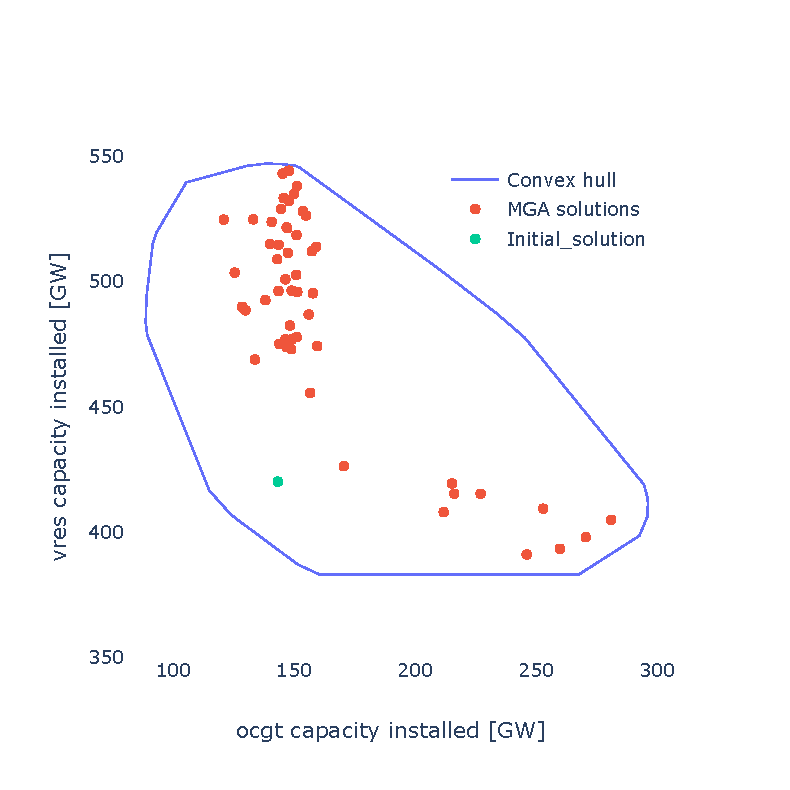
\includegraphics[width=1.\textwidth]{./Images/comparison_3}
		\caption{}
		\label{fig:comparison_4}
	\end{subfigure}
	\caption{On the figure the found MGA solutions within the reduced decision space of four MGA algorithms is presented. Figure (a) presents the results from the novel MGA method. Figure (b) shows the results from the maximization and minimization of grouped variables approach, as presented in \cite{Fabian_MGA}. Figure (c) presents results from the HSJ MGA method from \cite{DeCarolis_MGA}, and figure (d) shows the results from the maximization and minimization of all decision variables as presented in \cite{Fabian_MGA}.}
	\label{fig:comparison_results}
\end{figure}

Using the approach presented in section \ref{sec:dim_reduction} to reduce the dimensionality, a new two-dimensional decision space is formed, by grouping the variables in a group representing all installed gas turbine capacity and the other group representing all variable renewable energy source capacity (wind and solar power). This allows for easy visualization and understanding of the results. 

Initially the novel MGA approach presented in this project, was deployed to find the convex hull containing all solutions in the two-dimensional decision space. As this method converges towards the full solution, the result can be considered as the full solution to the two-dimensional problem. The found convex hull is presented in figure \ref{fig:comparison_1}. The shaded area of the convex hull indicates that the novel MGA approach extracts information about the entire hull volume in regard to all other MGA approaches that terminates when a set of different solution is found. Despite using a simplified techno-economic model and reducing dimensionality to just two dimensions, the shape of the convex hull is still rather complex. 

 



On figure \ref{fig:comparison_2}, the results of the method from \cite{Fabian_MGA} where the grouped decision variables are maximized and minimized, is presented. This method effectively performs the same initial MGA iteration as the novel MGA approach, and therefore it finds solutions also found be the novel MGA approach. In the work presented in \cite{Fabian_MGA}, these maximized and minimized solutions are used to create upper and lower bounds on the summarized capacities. Four individual solutions found using this technique is presented on figure \ref{fig:MGA_sum_results}. 


\begin{figure}[h]\centering
	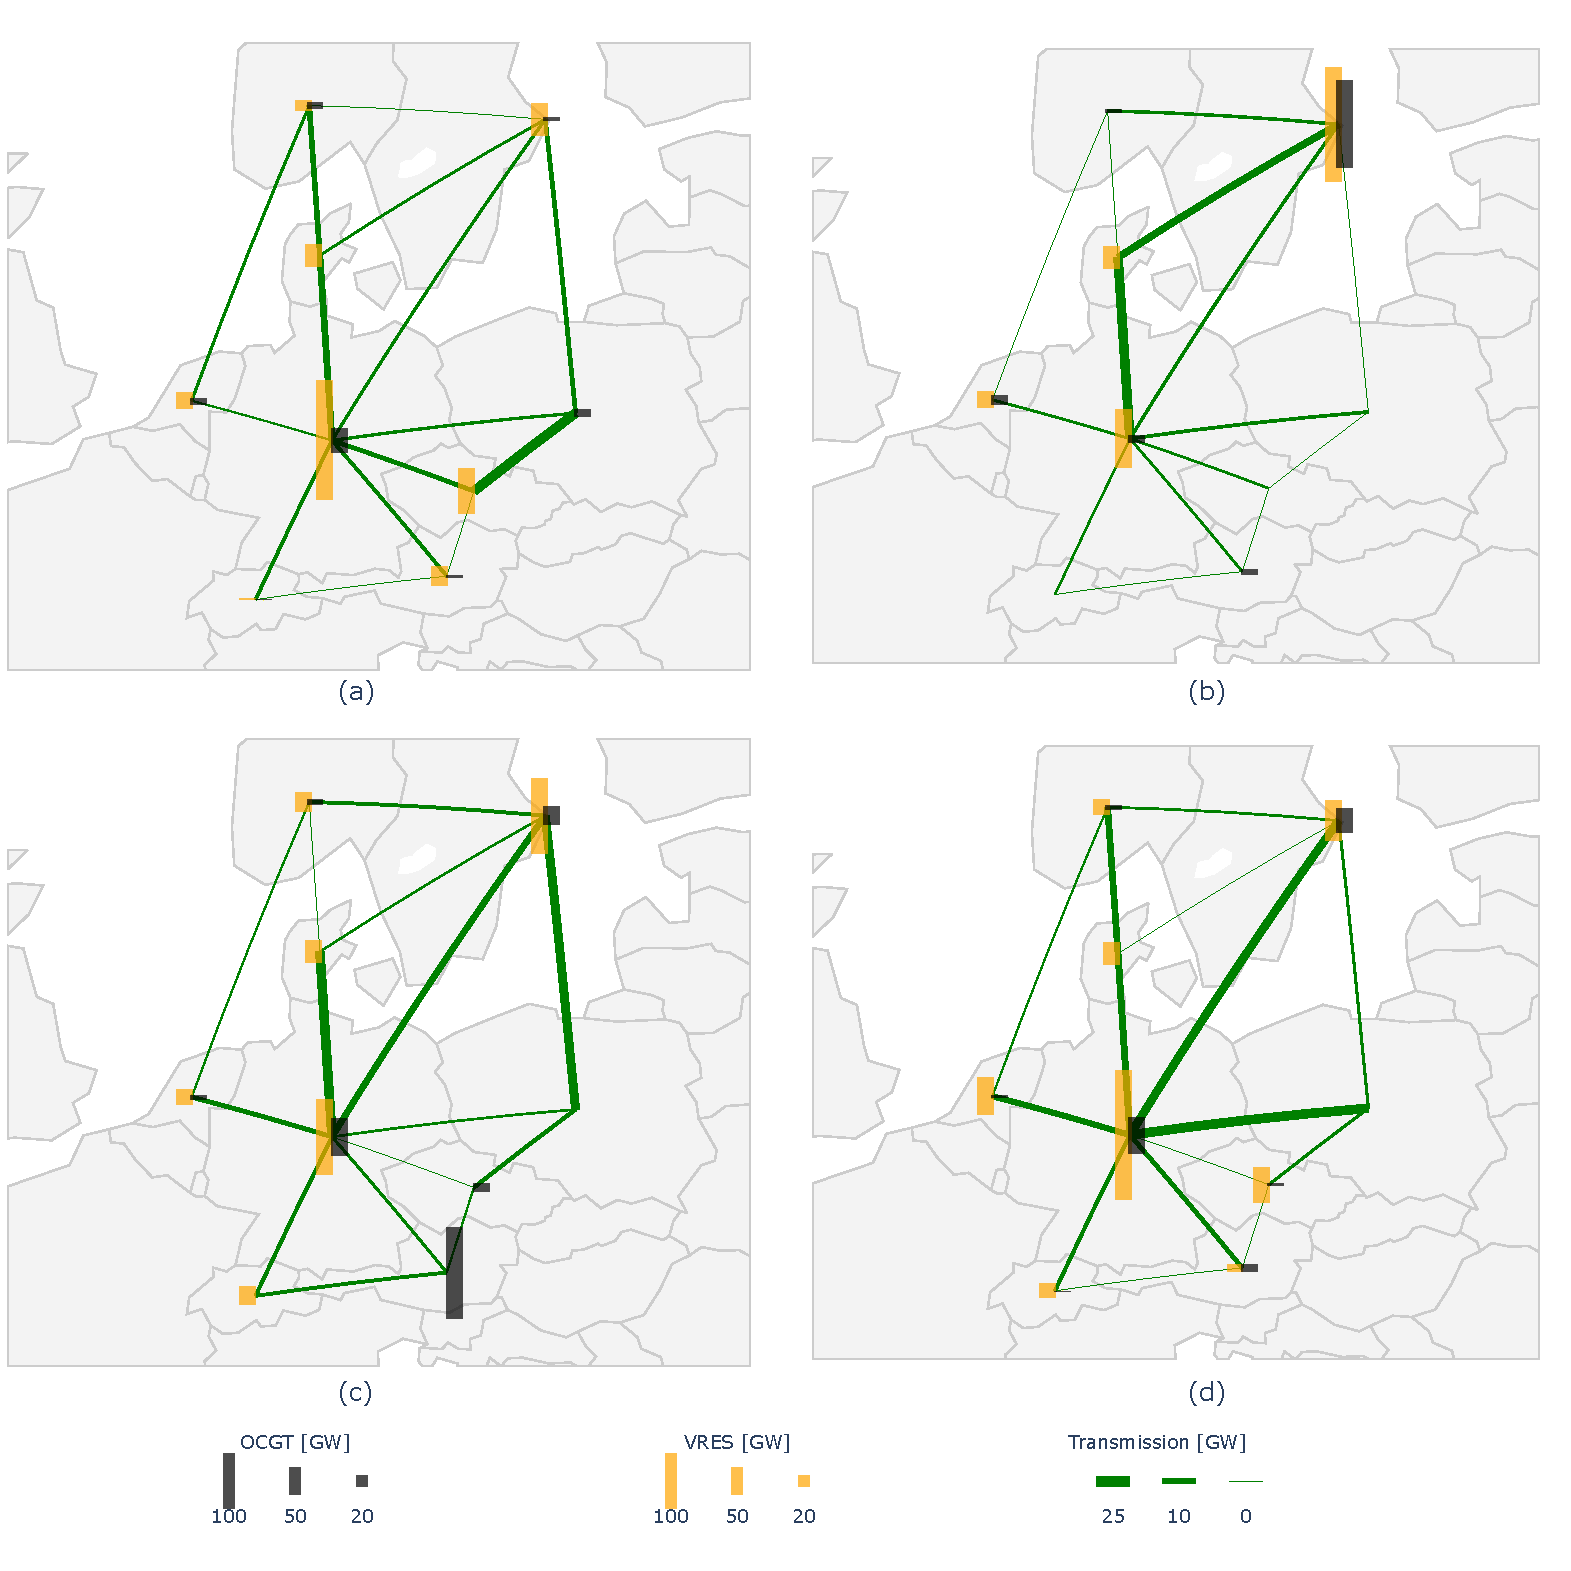
\includegraphics[width=1.\textwidth,trim={0 0cm 0 0cm},clip]{./Images/MGA_sum}
	\caption{On the figure a presentation of capacity distributions from four solutions using the novel MGA results is presented. The four studies have used the following objective functions: (a) Minimize OCGT, (b) Minimize VRES, (c) Maximize OCGT, (d) Maximize VRES}
	\label{fig:MGA_sum_results}
\end{figure}


Analyzing the result of the HSJ MGA method on figure \ref{fig:comparison_3}, it is clear that it does not search towards the edge of the convex hull as the first two methods. The reason hereof is that the HSJ method doesn't consider the grouped variables. Instead, it seeks to create maximally different solutions by implementing technologies not included in the previous solution. Here similar technologies from different countries are treated as two individual technologies. Analyzing the individual HSJ solutions presented on figure \ref{fig:HSJ_results} they are very different. Although all the solutions implement similar capacities of VRES and OCGT when summarized, the placement of the capacity implemented varies a lot from solution to solution. Looking at the two HSJ solutions from figure \ref{fig:HSJ_results}b and \ref{fig:HSJ_results}c, where solution (b) implements all VRES in Denmark and Germany, and solution (c) implements no VRES in Germany, but spreads it to the surrounding countries, it is easy to see that the solutions are topologically different but when analyzing the summarized capacities they are very similar. 

\begin{figure}[h]\centering
	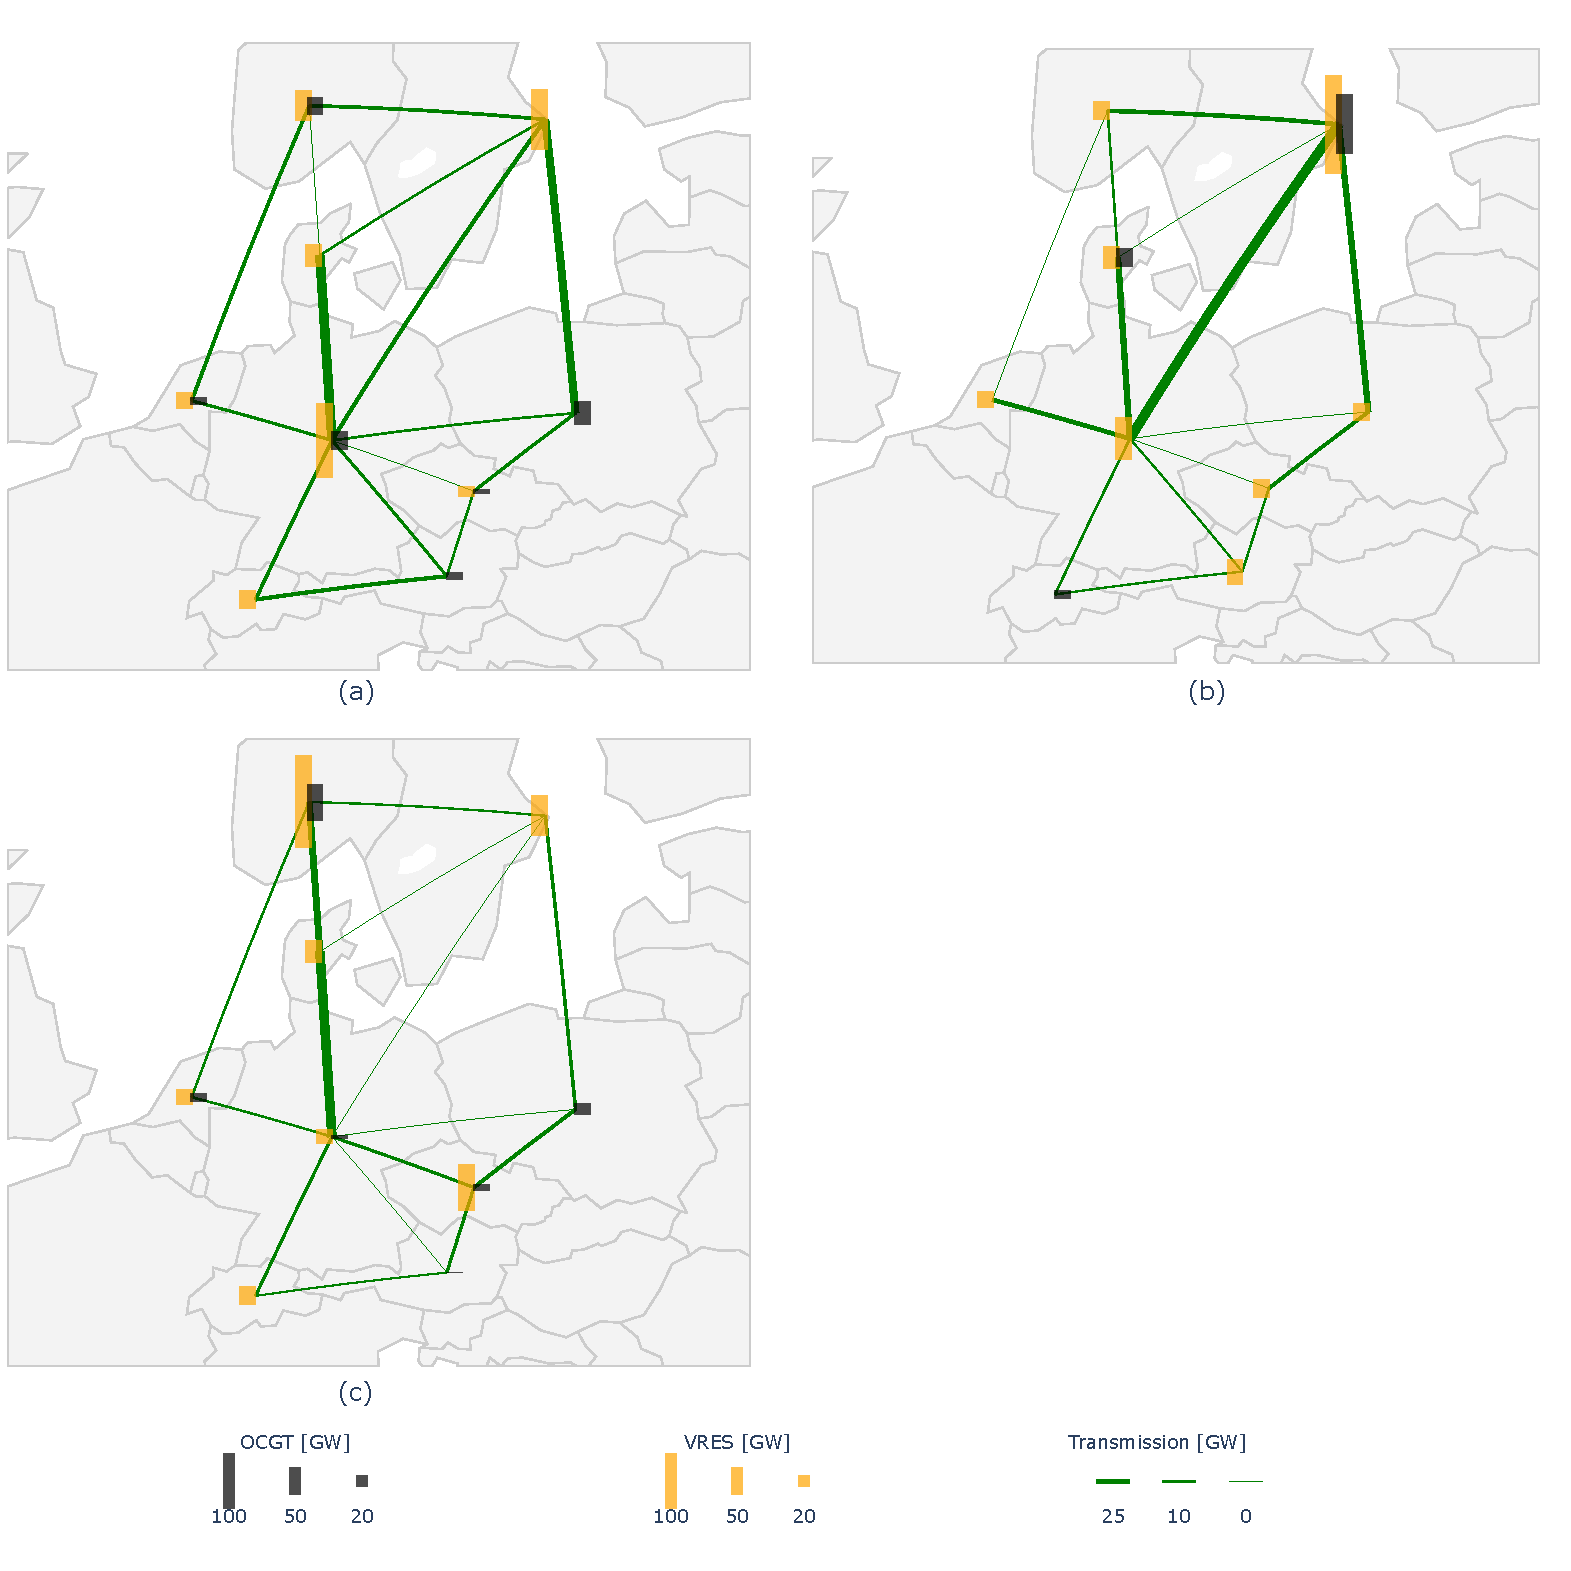
\includegraphics[width=1.\textwidth,trim={0 0cm 0 0cm},clip]{./Images/HSJ}
	\caption{On the figure a presentation of capacity distributions from three solutions using the novel HSJ MGA method is presented. Figure (a) shows the optimal solution, and figure (b) and (c) are HSJ solutions. }
	\label{fig:HSJ_results}
\end{figure}

The overall conclusion from this study must be that the novel MGA approach developed in this project shows to be very effective in its ability to determine the shape of the near optimal feasible space. Although it performs more optimizations than the other MGA methods, it uses these optimization runs wisely to investigate complex regions of the decision space. 


